\documentclass{article}
\usepackage{titlesec, geometry, setspace, enumitem, longtable, pdfpages, hyperref}

\hypersetup{
    colorlinks,
    citecolor=black,
    filecolor=black,
    linkcolor=black,
    urlcolor=black
}

\doublespacing

\geometry{
letterpaper,
textwidth=6.5in,
textheight=9in
}

\setlist{nosep}

\let\oldsection\section
\renewcommand\section{\clearpage\oldsection}

\renewcommand{\thesection}{\Roman{section}}
\titleformat
{\section}
[hang]
{\bfseries\Large}
{Section \thesection:} % label
{0.5em}{}

\renewcommand\thesubsection{\Alph{subsection}}
\titleformat{\subsection}
[hang]
{\large\bfseries}
{}{-1.1em}{}

\titlespacing{\subsection}{1.5em}{0em}{0em}

\begin{document}

\begin{titlepage}
\begin{center}
	\vspace*{1cm}
	\Huge
	\textbf{Online Retail Database}
	
	\vspace{1.5cm}
	\LARGE
	\textbf{Mark Kim}
	
	\Large
	Student ID: 918204214
	
	GitHub Username: mkim797
	
	\large
	\vspace{1cm}
	\begin{tabular}{ | l | c | }
		\hline
		\textbf{Milestone/Version} & \textbf{Date}\\
		\hline
		M1V1 & 09/11/2021\\
		\hline
	\end{tabular}

\end{center}
\end{titlepage}

\tableofcontents
\pagebreak

\section{Project Description}

The goal of this project is to design and implement an online retail database that functions similarly to the online portals of major retailers such as Walmart, The Home Depot, and Amazon.  This database system is to manage all aspects of online retail operations from product acquisition and warehousing, to customer order fulfillment and followup.  By implementing this database, the online retailer will be able to better understand product turnover, supply chain, human resourcing, fulfillment efficiency, and many other key performance indicators.

From the vendor side of the business, the database will manage the supply chain.  This will allow the business to ensure that its resources are applied as efficiently as possible.  The business will be able to understand how long it will take for each incoming order to be fulfilled so they can plan for the correct amount of warehouse space to be allocated for each order.  Additionally, the business will be able to choose multiple different vendors to aggregate supply capacity in the case that there are supply chain breakdowns.  This will minimize the chance for an interruption in the business's ability to fulfill orders to their customers.

Of course, as an online retail business, customers need to be carefully managed.  This database will facilitate the management of customer accounts, transactions, order fulfillment, and purchase habits.  By tracking these items, the business will be better equipped to manage their inventory, vendors, and sales trends.  By managing customer transactions, the business will be able to make informed decisions about how to manage its supply chain; the business will know how much of each product to order from its vendors.  As an added value to customers, the database will also allow customers to comment and review the products they order and their general experience with the business.

Lastly, and possibly most importantly, this project will manage internal operations.  This includes, but is not limited to, inventory management, warehousing and distribution, human resources and capital resources.  With this system, the business will be able to manage its staffing requirements and responsibilities, which warehouses to use when fulfilling customer orders, management and administrative hierarchy, and working capital.  This will allow the business to maintain smooth operations by ensuring proper staffing at all of its locations.  Furthermore, the business will be able to resource its distribution network to ensure timely and efficient fulfillment of orders.  Finally, the database will be able to support multiple roles for employees to ensure a separation of duties.

\section{Use Cases}
\subsection{Use Case 1}
\begin{description}[font=\bfseries\itshape]
\item[Title:]Product Purchase from Website
\item[Actors:]Customer (Leia Organa)
\item[Description:]Leia is someone who is looking for a new circular saw.  She is not happy with the last one she bought since it lacks the feature set she wants.  She wants to browse to see what kind of saws that the website has available.  She finds that there are categories that she can use to limit her search and since the saw is a type of tool, she chooses the tool category.  Nevertheless, tools have a lot more other subcategories, so she continues drilling down the menus until the list is limited to only circular saws.  Now that she has a nice succinct list of saws, she is able to compare them and find the one she wants.

\hspace*{2em}Once found, Leia adds the saw she wants to her shopping cart.  She continues browsing a little longer to see if there is anything else she wants, but decides that she doesn't need anything else and checks out.  After entering in her shipping address and billing address, she chooses a shipping method and completes the transaction.  Once completed, Leia receives an order confirmation email and when the item ships, she receives her receipt with all the relevant shipping details.
\end{description}

\subsection{Use Case 2}
\begin{description}[font=\bfseries\itshape]
\item[Title:]Product Order from Supplier
\item[Actors:]Buyer (Han Solo)
\item[Description:]Han is a buyer for the cutlery category of products at one of the warehouses of our online retailer.  Han's responsibilities include tracking sales and inventory so that he knows exactly what products to buy and when so that the retailer has enough supply to handle demand at any given moment.  There are many suppliers and manufacturers of cutlery, so he needs to ensure that fulfillment of the orders happen in a timely fashion.  If not, he needs to either find another supplier that can fulfill the order or find a substitute item that will satisfy the customers.  With all this in mind, Han logs into the system and checks the inventory of all the cutlery in stock at this warehouse.  He then contacts the supplier and orders many knives to be stocked in the warehouses.  He then enters the pending order in so that he can track the status of it.  Once completed, he continues ordering more cutlery from other vendors until he is sure that the warehouse will continue to have enough supply to handle demand.
\end{description}

\subsection{Use Case 3}
\begin{description}[font=\bfseries\itshape]
\item[Title:]Customer opens an account
\item[Actors:]Customer (Lando Calrissian)
\item[Description:]Lando shops at our online retailer regularly.  Because of this, he wants us to save his information to make his shopping experience more effortless.  He knows that once he opens an account, he can also sign up for our rewards program, where he can redeem points for credit on future purchases.  He is also aware of our premium subscription where he receives free expedited shipping for all his orders, but he is not sure if he wants to pay for this yet since he doesn't really need expedited shipping and all his orders qualify for free ground shipping anyways.

\hspace*{2em}Once he opens his account, he can save multiple shipping addresses and multiple payment methods, which allows him to purchase items quickly and effortlessly. He can also view all his purchase history and track the order status of all his orders.  Once he receives enough points in the rewards program, he can redeem the points for things like gift cards and special discounts or gifts.
\end{description}

\subsection{Use Case 4}
\begin{description}[font=\bfseries\itshape]
\item[Title:]Customer Order is Fulfilled
\item[Actors:]Warehouse Employee (Kylo Ren)
\item[Description:]This use case begins as Kylo goes to his station.  Once there, he logs into his computer terminal which shows him what orders he needs to box up and ship out. The computer terminal gives him the order number with a packing list of all the items to be packed up.  All the work of locating and pulling products has been automated, so his job is to double check the bin prepared by the robots and pack them securely in a box.  If there is an error, it is his responsibility to remove any incorrect products to be returned to the warehouse and request any products that may be missing.  Each of these errors are entered into the terminal along with any corrective action taken.  For example, if the warehouse shows that there is no inventory of a product, he must note that on his terminal so that it can either be fulfilled by another warehouse or notify the customer of a backorder or cancellation.  Once he verifies and packs all the items listed on his terminal, he completes the order by including a packing list inside and labeling the box with the shipping label provided to him.  Once he completes the order, he scans the box and sends it down the conveyor belt to be routed to the correct pickup area of the corresponding courier for delivery.
\end{description}

\subsection{Use Case 5}
\begin{description}[font=\bfseries\itshape]
\item[Title:]Product Return
\item[Actors:]Customer (Boba Fett), Warehouse Employee (Padme Amidala)
\item[Description:]Boba bought a microwave from the online retail store but it arrived broken, so she wants a replacement.  Since he is an account holder, he can log into his account and begin his return process from his order history.  After providing the reason for his return and once the system authorizes his return, he is given options for how he would like the return processed.  He chooses to get a replacement and bring the broken item to a participating brick and mortar retailer to pack and ship the product back because that is most convenient for him.  After completing the transaction, he is provided with a return ID that he is to supply the retailer along with the item to be returned.  He then gives the item to the retailer within the allowable time limit.  The retailer then scans the item, labels the return, and aggregates all the items that were received during the day to be picked up with a contracted courier to be returned to the closest warehouse.  Once the item is scanned, the fulfillment center creates a new order to replace the broken item.

\hspace*{2em}Once the warehouse receives the item, Padme is tasked with finishing the return process.  Padme already is logged into her work terminal.  She takes an item from the bin full of returns and scans it.  Once scanned, the item is flagged as received.  Padme then reviews the product and determines the cause of its inability to operate (i.e. damage from shipment, manufacturer defect, etc).  Once the cause is determined, she enters it into her terminal so that the correct entity is notified and corrective action is taken.
\end{description}

\section{Database Requirements}

\begin{enumerate}

\item General User (Strong)
\begin{enumerate}
	\item A general user shall create only one account with a unique email.
	\item A general user shall be able to register to many mailing lists
	\item A general user shall have many addresses
	\item A general user shall have many payment methods
	\item A general user shall create many orders
	\item A general user is a registered user
\end{enumerate}
	
\item Registered User (Strong - Recursive)
\begin{enumerate}
	\item A registered user is a general user.
	\item A registered user shall be allowed to login to their account from many supported devices simultaneously.
\end{enumerate}
	
\item Device (Strong)
\begin{enumerate}
	\item A device shall log into zero or one account
	\item A device shall be used by many registered users
\end{enumerate}

\item Account
\begin{enumerate}
	\item An account shall be created by one and only one user
	\item An account is a Basic Account
	\item An account is a Premium Account
	\item An account shall be logged into by many devices
	\item An account shall accrue at least one reward
\end{enumerate}
	
\item Basic Account
\begin{enumerate}
	\item A Basic account is an account
\end{enumerate}
	
\item Premium Account
\begin{enumerate}
	\item A Premium account is an account
\end{enumerate}

\item Reward (Strong)
\begin{enumerate}
	\item A reward shall be accrued by many accounts
\end{enumerate}
	
\item Mailing List (Strong)
\begin{enumerate}
	\item A mailing list shall have many users
\end{enumerate}

\item Order (Weak)
\begin{enumerate}
	\item An order is a purchase
	\item An order is a return
	\item An order ships to at most one shipping address
	\item An order has one order details
	\item An order creates at least one fulfillment action
\end{enumerate}

\item Purchase
\begin{enumerate}
	\item A purchase is an order
\end{enumerate}

\item Return
\begin{enumerate}
	\item A return is an order
\end{enumerate}

\item Order Details (Weak)
\begin{enumerate}
	\item An order detail generates one receipt
	\item An order detail receives payment from at least one payment method
	\item An order detail contains at least one product
	\item An order detail sends payment details to one accounting department
\end{enumerate}
	
\item Receipt
\begin{enumerate}
	\item A receipt shall be generated by one and only one order details
\end{enumerate}
	
\item Accounting Dept (Strong)
\begin{enumerate}
	\item An accounting dept shall receive payment details from many order details
	\item An accounting dept shall pay many payees
\end{enumerate}

\item Payee (Strong)
\begin{enumerate}
	\item A payee shall be payed by many accounting departments
\end{enumerate}
	
\item Address (Strong)
\begin{enumerate}
	\item An address shall be associated with many general users
	\item An address is a billing address
	\item An address is a primary address
	\item An address is a shipping address
\end{enumerate}
	
\item Primary Address
\begin{enumerate}
	\item A primary address is an address
\end{enumerate}
	
\item Billing Address
\begin{enumerate}
	\item A billing address is an address
	\item A billing address has at least one payment method
\end{enumerate}
	
\item Shipping Address
\begin{enumerate}
	\item A shipping address is an address
	\item A shipping address is shipped to by many orders
\end{enumerate}

\item Payment method (Strong)
\begin{enumerate}
	\item A payment method is a Bank Account
	\item A payment method is a Credit Card
	\item A payment method is Cryptocurrency
	\item A payment method pays for many orders
	\item A payment method has one billing address
	\item A payment method has at most one general user
\end{enumerate}
	
\item Bank Account
\begin{enumerate}
	\item A bank account is a payment method
	\item A bank account is a checking account
	\item A bank account is a savings account
\end{enumerate}
	
\item Checking account
\begin{enumerate}
	\item A checking account is a bank account
\end{enumerate}
	
\item Savings account
\begin{enumerate}
	\item A saving account is a bank account
\end{enumerate}
	
\item Credit card
\begin{enumerate}
	\item A credit card is a payment method
\end{enumerate}
	
\item Crypto
\begin{enumerate}
	\item Crypto is a payment method
\end{enumerate}
	
\item Fulfillment Action (Strong)
\begin{enumerate}
	\item A fulfillment action is created by many orders
	\item A fulfillment action uses at most one courier
	\item A fulfillment action has at most one region
\end{enumerate}
	
\item Region (Strong)
\begin{enumerate}
	\item A region has many fulfillment actions
	\item A region has many warehouses
\end{enumerate}

\item Courier (Strong)
\begin{enumerate}
	\item A courier is used by many fulfillment actions
\end{enumerate}
	
\item Warehouse (weak?)
\begin{enumerate}
	\item A warehouse has one region
	\item A warehouse requests many inventory items from many suppliers
\end{enumerate}

\item Product (Strong)
\begin{enumerate}
	\item A product is ordered from many order details
	\item A product is stocked in many inventories
	\item A product has many categories
	\item A product has many promotions
\end{enumerate}

\item Promotion (Strong)
\begin{enumerate}
	\item A promotion is associated with many products
\end{enumerate}

\item Category (Strong)
\begin{enumerate}
	\item A category has many products
\end{enumerate}

\item Inventory (Strong)
\begin{enumerate}
	\item An inventory contains many products
	\item An inventory receives many items from many suppliers
	\item An inventory stocks many warehouses
\end{enumerate}

\item Supplier (Strong)
\begin{enumerate}
	\item A supplier sends many items to inventory
	\item A supplier is requested by a warehouse to send many items
\end{enumerate}

\end{enumerate}

\section{Detailed List of Main Entities, Attributes and Keys}

\begin{enumerate}
\item General User (Strong)
    \begin{itemize}
        \item user\_id: key, numeric
        \item name: composite, alphanumeric
        \item email: alphanumeric
        \item phone: numeric
    \end{itemize}
\item Registered User (Strong)
    \begin{itemize}
        \item registered\_user\_id: key, numeric
        \item login: alphanumeric
        \item account\_id: foreign key, numeric
    \end{itemize}
\item Address (Strong)
    \begin{itemize}
        \item address\_id: key, numeric
        \item address: composite, alphanumeric
        \item city: alphanumeric
        \item state: alphanumeric
        \item zip\_code: numeric
        \item country: alphanumeric
        \item address\_type: numeric
    \end{itemize}
\item Device (Strong)
    \begin{itemize}
        \item device\_id: key, numeric
        \item device\_type: alphanumeric
        \item device\_os: alphanumeric
        \item device\_ip: numeric
    \end{itemize}
\item Mailing List (Strong)
    \begin{itemize}
        \item mailinglist\_id: key, numeric
        \item mailinglist\_name: alphanumeric
        \item description: alphanumeric
        \item mailinglist\_category: alphanumeric
    \end{itemize}
\item Account (Weak)
    \begin{itemize}
        \item account\_id: key, numeric
        \item registered\_user\_id: foreign key, numeric
        \item account\_type: numeric
    \end{itemize}
\item Region (Strong)
    \begin{itemize}
        \item region\_id: key, numeric
        \item location: composite, alphanumeric
        \item service\_area: numeric
    \end{itemize}
\item Promotion (Strong)
    \begin{itemize}
        \item promotion\_id: key, numeric
        \item promotion\_type: numeric (e.g. discount, free item, etc)
        \item promotion\_limit: numeric (e.g. applies only once, or maximum 3 items, etc)
    \end{itemize}
\item Reward (Strong)
    \begin{itemize}
        \item reward\_id: key, numeric
        \item reward\_type: numeric (e.g. discount, free item, etc)
        \item reward\_limit: numeric (e.g. applies only once, or maximum 3 items, etc)
    \end{itemize}
\item Payment Method (Strong)
    \begin{itemize}
        \item payment\_id: key, numeric
        \item billing\_address\_id: foreign key, numeric
        \item payment\_type: alphanumeric
    \end{itemize}
\item Order (Weak)
    \begin{itemize}
        \item order\_id: key, numeric
        \item user\_id: foreign key, numeric
        \item shipping\_address\_id: foreign key, numeric
        \item order\_type: numeric
    \end{itemize}
\item Order Details (Weak)
    \begin{itemize}
        \item order\_details\_id: key, numeric
        \item order\_id: foreign key, numeric
        \item payment\_method\_id: foreign key, numeric
        \item receipt\_id: foreign, numeric
    \end{itemize}
\item Receipt (Weak)
    \begin{itemize}
        \item receipt\_id: key, numeric
        \item order\_details\_id: key, numeric
        \item receipt\_generated: timestamp
    \end{itemize}
\item Product (Strong)
    \begin{itemize}
        \item product\_id: key, numeric
        \item UPC\_code: unique, numeric
        \item product\_name: alphanumeric
        \item product\_description: alphanumeric
        \item product\_price: numeric
        \item product\_cost: numeric
    \end{itemize}
\item Category (Strong)
    \begin{itemize}
        \item category\_id: key, numeric
        \item category\_name: alphanumeric
        \item category\_description: alphanumeric
    \end{itemize}
\item Inventory (Strong)
    \begin{itemize}
        \item inventory\_id: key, numeric
        \item category\_name: alphanumeric
        \item category\_description: alphanumeric
    \end{itemize}
\item Supplier (Strong)
    \begin{itemize}
        \item supplier\_id: key, numeric
        \item location: multivalue, alphanumeric
        \item description: alphanumeric
    \end{itemize}
\item Warehouse (Weak)
    \begin{itemize}
        \item warehouse\_id: key, numeric
        \item region\_id: foreign key, numeric
        \item location: multivalue, alphanumeric
    \end{itemize}
\item Fulfillment Action (Strong)
    \begin{itemize}
        \item fulfillment\_id: key, numeric
        \item order\_id: foreign key, numeric
        \item package\_dimensions: composite, numeric
        \item package\_weight: numeric
        \item shipping\_priority: alphanumeric
        \item fulfillment\_status: numeric
    \end{itemize}
\item Courier (Strong)
    \begin{itemize}
        \item courier\_id: key, numeric
        \item courier\_account\_id: alphanumeric
        \item service\_area: alphanumeric
        \item service\_limit: alphanumeric (e.g. maximum/minimum package size/weight)
    \end{itemize}
\item Accounting Dept (Strong)
    \begin{itemize}
        \item accounting\_dept\_id: key, numeric
        \item order\_details\_id: foreign key, numeric
        \item payment\_date: timestamp
    \end{itemize}
\item Payees (Strong)
    \begin{itemize}
        \item payee\_id: key, numeric
        \item payment\_amount: numeric
        \item payment\_status: alphanumeric
    \end{itemize}
\end{enumerate}


\section{Entity Relationship Diagram (ERD)}
\begin{figure}
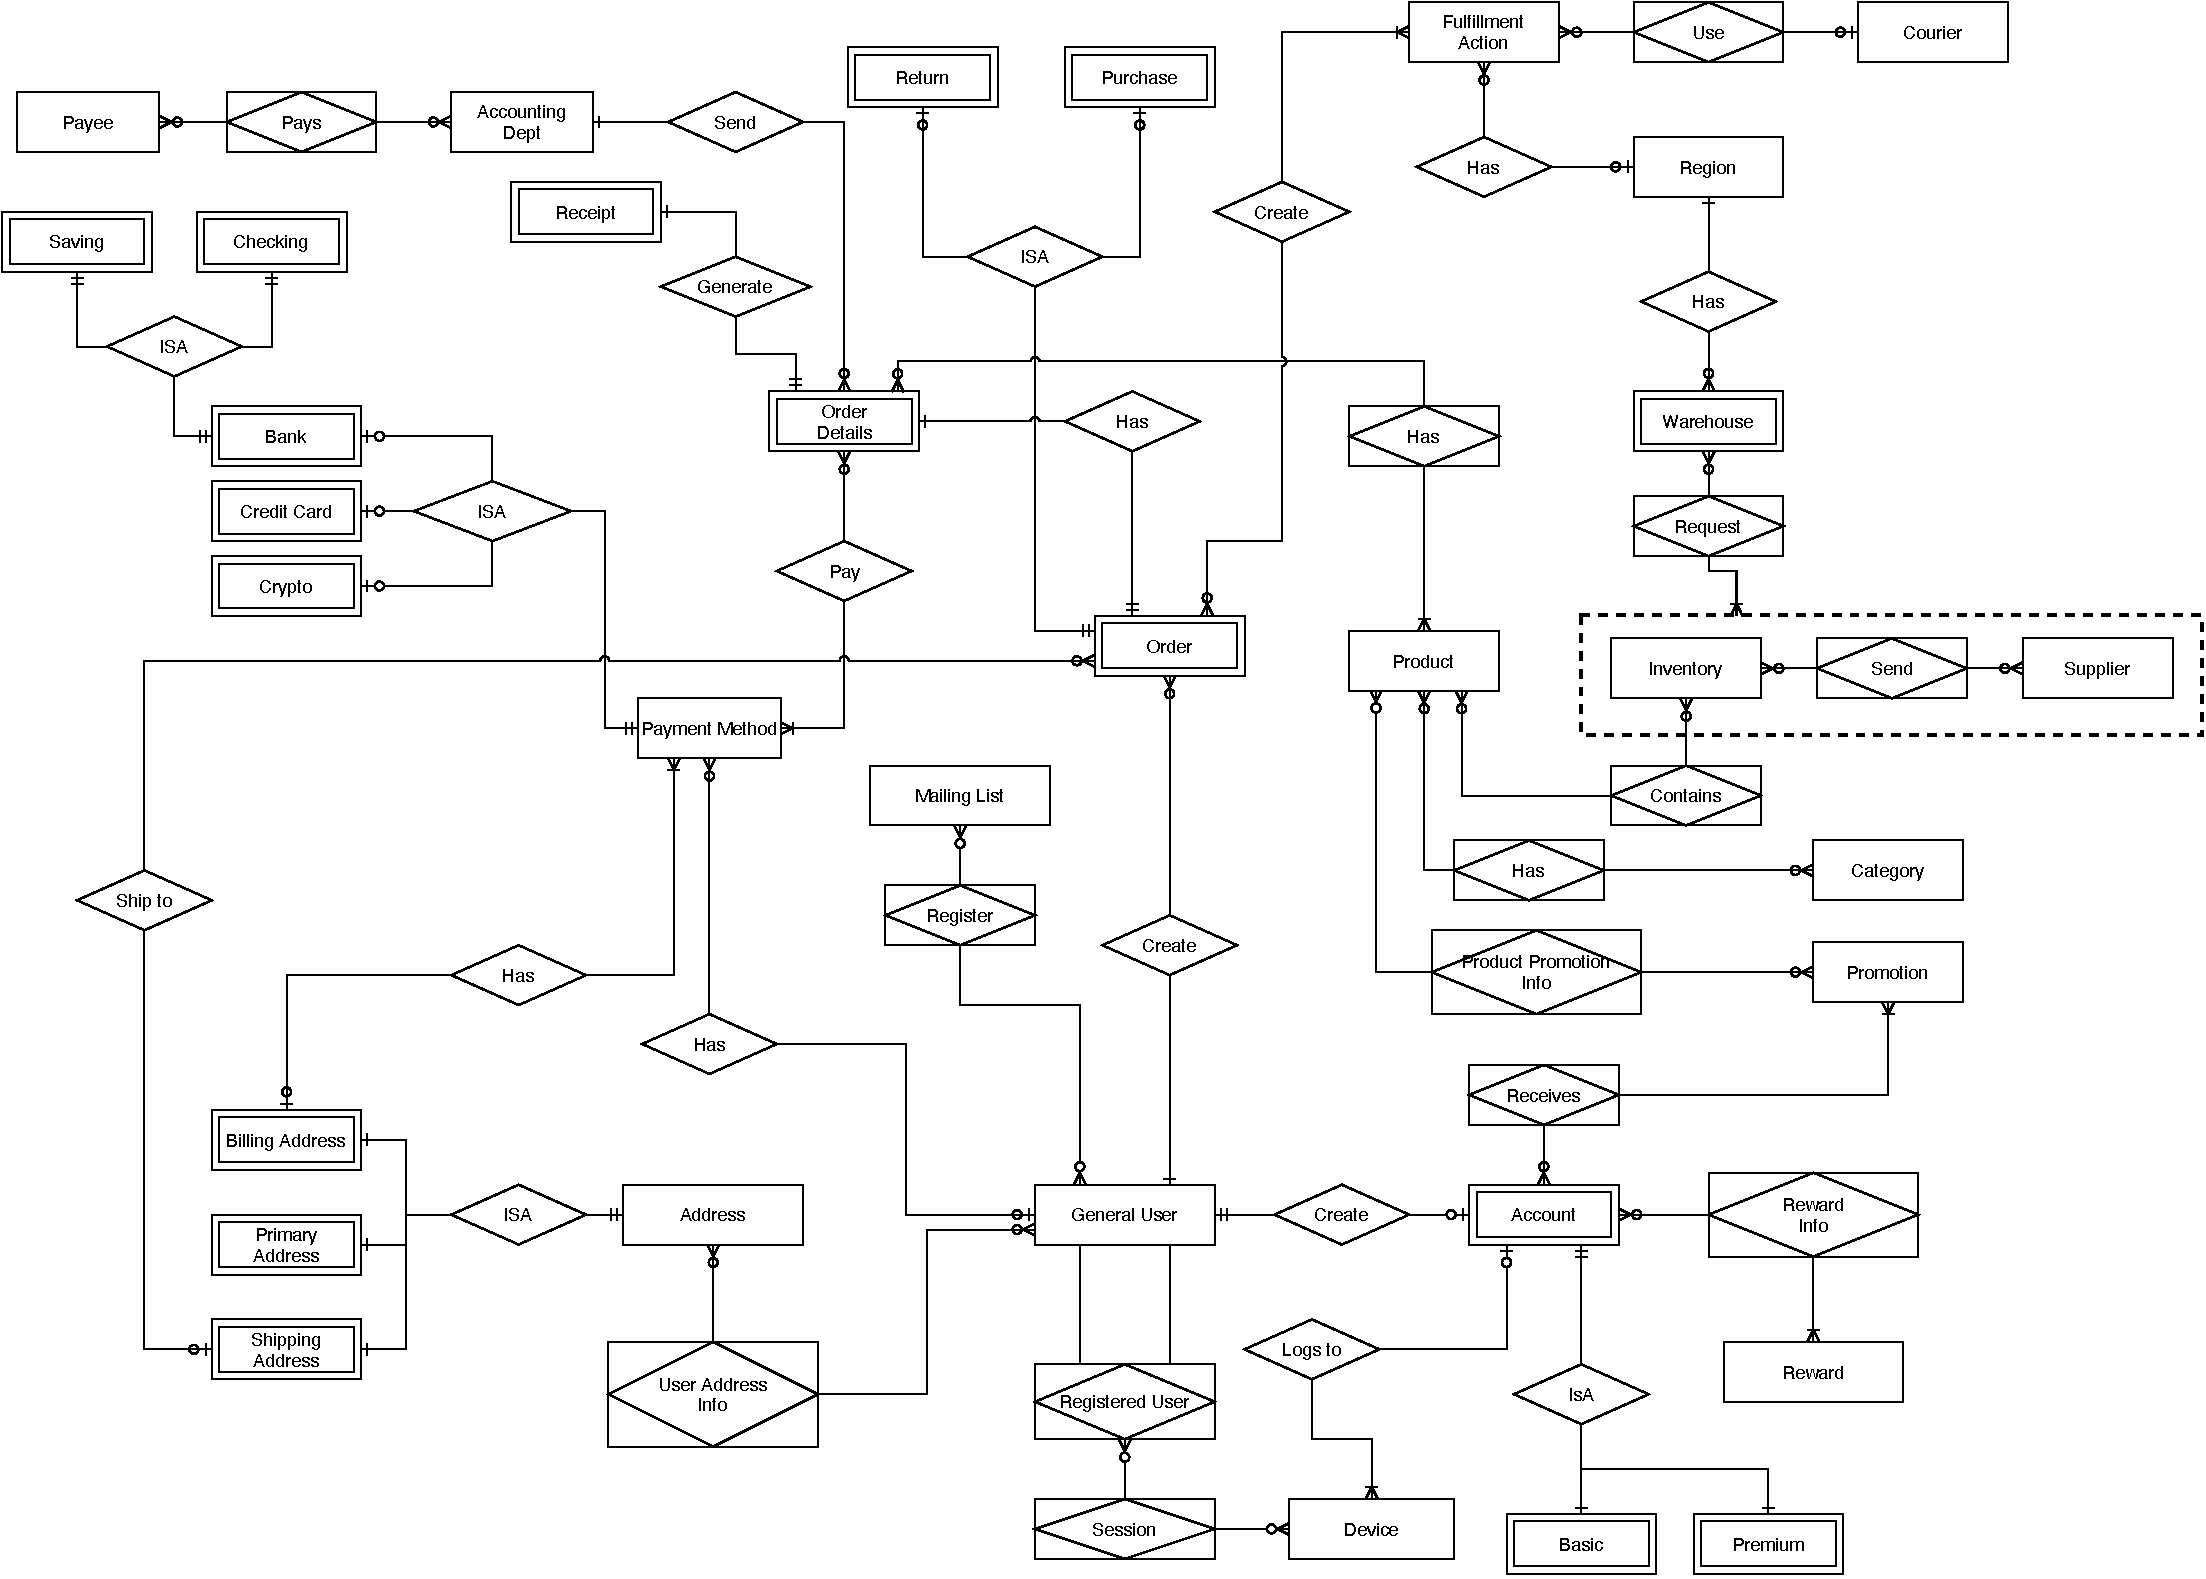
\includepdf[scale= 0.74, angle=90, pagecommand={\thispagestyle{plain}}]{OnlineRetailDB.drawio.pdf}
\end{figure}

\section{Testing Table}

\begin{longtable}{ | c | p{0.1\linewidth} | p{0.1\linewidth} | p{0.1\linewidth} | p{0.1\linewidth} | p{0.1\linewidth} | p{0.3\linewidth} | }
	\hline
	Rule & Entity A & Relation & Entity B & Cardinality & Pass/Fail & Error Description\\\hline\endhead
	1	 & General User & Create & Account & 1-to-1 & Pass & None \\\hline
	2	 & General User	& User Address Info & Address	& M-to-M	& Pass	& None \\\hline
	3	 & General User & User Payment Info	& Payment Method	& M-to-M	& Fail & A payment method should be associated with at most one user.  If a payment method can be associated with several users, there could be security issues.\\\hline
	4	 & General User & Registers	& Mailing List	& M-to-M	& Pass & None \\\hline
	5	 & General User & Creates	& Order	& 1-to-1	& Fail & A user should be able to order more than once. \\\hline
	6	 & Registered User & Open Session & Device & 1-to-M	&	Fail & Device can be used by multiple users. \\\hline
	7	& Device & Logs to & Account & M-to-1 & Fail & Device does not necessarily have to be logged in.  Can't force a device to be logged in. \\\hline
	8	& Account & Reward Info & Reward & M-to-M & Pass & None\\\hline
	9	& Account & Receives & Promotion & M-to-M & Pass & None\\\hline
	10	& Order & Ships to & Shipping Address & 1-to-1 & Fail & A single order should be shipped to at most one shipping address.  To ship to a different address, another order should be generated.  Also, the shipping address does not have to be shipped to by an order.\\\hline
	11	& Order & Has & Order Details & M-to-M & Fail & A single order should have only one order detail associated with it.  An order detail should be associated with one and only one order.\\\hline
	12	& Order & Create & Fulfillment action & M-to-M & Pass & None\\\hline
	13	& Order Details & Payed by & Payment Method & M-to-M & Pass & None\\\hline
	14	& Order Details & Generate & Receipt & 1-to-1 & Pass & None\\\hline
	15	& Order Details & Send & Accounting Dept & M-to-M & Fail & Order details must send details to one accounting department.  And Accounting department does not necessarily have to receive details from Order details.\\\hline
	16	& Order Details & Has & Product & M-to-M & Pass & None\\\hline
	17	& Fulfillment action & Use & Courier & M-to-M & Fail & A fulfillment action should use at most one courier.\\\hline
	18	& Fulfillment action & Has & Region & M-to-M & Fail & A fulfillment action should be associated with at most one region\\\hline
	19	& Region & Has & Warehouse & 1-to-M & Pass & None \\\hline
	20	& Warehouse & Requests & Inventory & M-to-M & Pass & None \\\hline
	21	& Warehouse & Requests from & Supplier & M-to-M & Pass & None \\\hline
	22	& Product & Contains & Inventory & M-to-M & Pass & None \\\hline
	23	& Product & Has & Category & M-to-M & Pass & None \\\hline
	24	& Product & Promotion Info & Promotion & M-to-M & Pass & None\\\hline
	25	& Supplier & Sends & Inventory & M-to-M & Pass & None \\\hline
	26	& Accounting Dept & Pays & Payees & M-to-M & Pass & The accounting department should not be forced to be paying payees, but payees do not require the accounting department to always be paying them.\\\hline
\end{longtable}

\end{document}